\section{Расчет второго вириального коэффициента и квантовых поправок}

\subsection{Групповое разложение}

Рассмотрим однокомпонентный классический газ, состоящий из $N$ одинаковых частиц и занимающих объем $V$. Предположим, что парные взаимодействия частиц являются центральными, и общая потенциальная энергия $U$ является суммой парных взаимодействий частиц $u = u(r)$. В таком случае полная потенциальная энергия системы может быть записана в виде $U \lb \mathbf{r}^N \rb = \displaystyle \dfrac{1}{2} \sum_{i, j} u_{ij}$, где $u_{ij}$ -- потенциал взаимодействия для изолированной пары молекул (Это предположение справедливо, за исключением случаев молекул, имеющих тенденцию к ассоциированию.). Конфигурационный интеграл газа $Z_N$ запишется в виде:
\vverh
\begin{gather}
	Z_N (T, V) = \int_V \cdots \int_V \exp \lb - \frac{\displaystyle\sum_{1 \leqslant i < j \leqslant N} u \lb r_{ij} \rb}{kT} \rb d \mathbf{r}_1 d \mathbf{r}_2 \dots \mathbf{r}_N = \notag \\
	= \int_V \cdots \int_V \prod_{1 \leqslant i < j \leqslant N} \exp \lb - \frac{u \lb r_{ij} \rb}{KT} \rb d \mathbf{r}_1 d \mathbf{r}_2 \dots d \mathbf{r}_N \label{confint}
\end{gather}

Функция Майера определена соотношением
\vverh
\begin{gather}
	\exp \lb - \frac{u \lb r_{ij} \rb}{kT} \rb = 1 + f_{ij} . \label{mayer}
\end{gather}
Функция $f = f(r)$ обладает следующими общими свойствами в зависимости от расстояния: при $r \longrightarrow 0: f(r) \longrightarrow -1$, затем $f(r)$ монотонно возрастает, проходит через максимум при расстоянии $r = d_0$, отвечающему минимуму потенциала $u(r)$, и при дальнейшем увеличении растояния между частицами она монотонно убывает, $f(r) \longrightarrow 0$ при $r \longrightarrow \infty$, оставаясь положительной. Таким образом, функция Майера существенно отлична от нуля только при расстояниях, отвечающих достаточно близкому расположению частиц. Подставляя выражение \eqref{mayer} в выражение для конфигурационного интеграла \eqref{confint}, получаем
\vverh
\begin{gather}
	Z_N (T, V) = \int_V \cdots \int_V \prod_{1 \leqslant i < j \leqslant N} \lb 1 + f_{ij} \rb d \mathbf{r}_1 d \mathbf{r}_2 \dots d \mathbf{r}_N , \label{confint1}
\end{gather}
в которой подынтегральное выражение есть произведение $\displaystyle\frac{N \lb N - 1 \rb}{2}$ функций $\lb 1 + f_{ij} \rb$, каждая из которых соответсвует определенной паре частиц. Раскрывая произведение в \eqref{confint1}, получаем
\vverh
\begin{gather}
	Z_N = \int_V \cdots \int_V \lb 1 + \sum_{i < j} f_{ij} + \sum_{i, j} \sum_{k,l} f_{ij} f_{kl} + \dots \rb d \mathbf{r}_1 d \mathbf{r}_2 \dots d \mathbf{r}_N = \int_V \cdots \int_V d \mathbf{r}_1 d \mathbf{r}_2 \dots d \mathbf{r}_N + \notag \\ 
	+ \sum_{i < j} \int_V \cdots \int_V f_{ij} d \mathbf{r}_1 d \mathbf{r}_2 \dots d \mathbf{r}_N + \sum_{i, j} \sum_{k, l} \int_V \cdots \int_V f_{ij} f_{kl} d \mathbf{r}_1 d \mathbf{r}_2 \dots d \mathbf{r}_N + \dots \label{confint2}  
\end{gather}

\subsection{$N$-частичные графы}
Каждому члену в разложении \eqref{confint2} можно сопоставить $N$-частичный граф, состоящий из $N$ пронумерованных вершин, соединенных ребрами в том случае, если в подынтегральном выражении функция Майера, содержащая индексы рассматриваемых вершин. Для $6$-частичного графа имеем

\begin{figure}[h]
\centering
\begin{minipage}{0.3\linewidth}
	\begin{tikzpicture}
	[vertex/.style={circle, draw=blue!50, fill=blue!20, thick}]
	\node[vertex] (1) {1};
	\node[vertex] (2) [below = 1cm of 1] {2}
		edge [thick] (1);
	\node[vertex] (3) [right = 1cm of 1] {3};
	\node[vertex] (4) [below = 1cm of 3] {4};
	\node[vertex] (5) [right = 1cm of 3] {5}
		edge [thick] (4);
	\node[vertex] (6) [below = 1 cm of 5] {6}
		edge [thick] (5);
	\begin{scope}[on background layer]
		\node [fill=yellow!20,fit=(1) (2) (5) (6)] {};
	\end{scope}
	\end{tikzpicture}
\end{minipage}%
\begin{minipage}{0.5\linewidth}
		\begin{equation*}
			\int \cdots \int f_{12} f_{45} f_{56} \, d \mathbf{r}_1 d \mathbf{r}_2 \dots d \mathbf{r}_6
		\end{equation*}
\end{minipage}
\caption{Пример $6$-частичного интеграла и соответствующего графа. }
\end{figure}

Назовем $l$-группой такой $l$-частичный граф, в котором к каждой вершине подходит по крайней мере одно ребро ($l$-группа -- связный $l$-частичный граф). Очевидно
\vverh
\begin{gather}
	\sum_l l m_l = N \label{cond1}
\end{gather}
Обозначим через $m_l$ число $l$-групп для данного $N$-частичного графа, являющегося членом разложения конфигурационного интеграла $Z_N$. Данному набор чисел $\left\{ m_l \right\} = \left\{ m_1 , m_2 , \dots, m_N \right\}$, $( m_l \geqslant 0 )$ отвечает некоторая совокупность $N$-графов, сумму которых обозначим через $S_N \left( \left\{ m_l \right\} \right)$, тогда:
\vverh
\begin{gather}
	Z_N = \sum_{ \left\{ m_l \right\} } S_N \left( \left\{ m_l \right\} \right), \label{confsum}
\end{gather}
где суммирование проводится по всем наборам чисел $\left\{ m_l \right\}$, удовлетворяющих условию \eqref{cond1}. \par
Диаграммы, образующие $S_N \left( \left\{ m_l \right\} \right)$, отличаются, во-первых, способом распределения пронумерованных частиц по группам. Во-вторых, $l$-группы при $l \geqslant 3$ могут быть составлены из данных пронумерованных частиц различными способами. Так, при $N=4$, $m_1 = 1$, $m_2 = 0$, $m_3 = 1$, при распределении пронумерованных частиц $1; 2-3-4$ будут различными следующие четыре диаграммы:
\vverh
\begin{figure}[h]
	\begin{minipage}{0.33\linewidth}
		\begin{tikzpicture}
			[vertex/.style={circle, draw=blue!50, fill=blue!20, thick}]
			\node (dummy) {};
			\node[vertex] (1) [below = -0.1cm of dummy] {1};
			\node[vertex] (2) [below right = 1cm and 1.3cm of dummy] {2};
			\node[vertex] (3) [above right = 1cm and 0.6cm of 2] {3}
				edge [thick] (2); 
			\node[vertex] (4) [below right = 1cm and 0.6cm of 3] {4}
				edge [thick] (3);
			\begin{scope}[on background layer]
				\node [fill=yellow!20,fit=(1) (2) (3) (4)] {};
			\end{scope}
		\end{tikzpicture}
		\caption*{$\displaystyle\int d \mathbf{r}_1 \int \int \int f_{23} f_{34} \, d \mathbf{r}_2 d \mathbf{r}_3 d \mathbf{r}_4$}
	\end{minipage}
	\begin{minipage}{0.33\linewidth}
		\begin{tikzpicture}
			[vertex/.style={circle, draw=blue!50, fill=blue!20, thick}]
			\node (dummy) {};
			\node[vertex] (1) [below = -0.1cm of dummy] {1};
			\node[vertex] (2) [below right = 1cm and 1.3cm of dummy] {2};
			\node[vertex] (3) [above right = 1cm and 0.6cm of 2] {3}
				edge [thick] (2); 
			\node[vertex] (4) [below right = 1cm and 0.6cm of 3] {4}
				edge [thick] (2);
			\begin{scope}[on background layer]
				\node [fill=yellow!20,fit=(1) (2) (3) (4)] {};
			\end{scope}
		\end{tikzpicture}
		\caption*{$\displaystyle \int d \mathbf{r}_1 \int \int \int f_{23} f_{24} \, d \mathbf{r}_2 d \mathbf{r}_3 d \mathbf{r}_4$}
	\end{minipage}
	\begin{minipage}{0.33\linewidth}
		\begin{tikzpicture}
			[vertex/.style={circle, draw=blue!50, fill=blue!20, thick}]
			\node (dummy) {};
			\node[vertex] (1) [below = -0.1cm of dummy] {1};
			\node[vertex] (2) [below right = 1cm and 1.3cm of dummy] {2};
			\node[vertex] (3) [above right = 1cm and 0.6cm of 2] {3};
			\node[vertex] (4) [below right = 1cm and 0.6cm of 3] {4}
				edge [thick] (3)
				edge [thick] (2);
			\begin{scope}[on background layer]
				\node [fill=yellow!20,fit=(1) (2) (3) (4)] {};
			\end{scope}
		\end{tikzpicture}
		\caption*{$\displaystyle \int d \mathbf{r}_1 \int \int \int f_{24} f_{34} \, d \mathbf{r}_2 d \mathbf{r}_3 d \mathbf{r}_4$}
	\end{minipage} \\
	\begin{center}
	\begin{minipage}{0.33\linewidth}
		\begin{tikzpicture}
			[vertex/.style={circle, draw=blue!50, fill=blue!20, thick}]
			\node (dummy) {};
			\node[vertex] (1) [below = -0.1cm of dummy] {1};
			\node[vertex] (2) [below right = 1cm and 1.3cm of dummy] {2};
			\node[vertex] (3) [above right = 1cm and 0.6cm of 2] {3}
				edge [thick] (2);
			\node[vertex] (4) [below right = 1cm and 0.6cm of 3] {4}
				edge [thick] (3)
				edge [thick] (2);
			\begin{scope}[on background layer]
				\node [fill=yellow!20,fit=(1) (2) (3) (4)] {};
			\end{scope}
		\end{tikzpicture}
		\caption*{$\displaystyle \int d \mathbf{r}_1 \int \int \int f_{23} f_{24} f_{34} \, d \mathbf{r}_2 d \mathbf{r}_3 d \mathbf{r}_4$}
	\end{minipage}
\end{center}
\caption{Четыре варианта $3$-групп при $N = 4$ и фиксированном распределении $1; 2, 3, 4$ с соответствующими интегралами.}
\end{figure}

Если число $l$-групп равно $m_l$, то они дают сомножитель, дающий вклад в $S_N \lb \left\{ m_l \right\} \rb$, который будем обозначать $\bigg[ \text{сумма всех $l$-групп} \bigg]^m_l$. Так 3-группы дают сомножитель
\vverh
\begin{gather}
\int d \mathbf{r}_1 \int \int \int f_{23} f_{34} \, d \mathbf{r}_2 d \mathbf{r}_3 d \mathbf{r}_4 + $ $+ \displaystyle \int d \mathbf{r}_1 \int \int \int f_{23} f_{24} \, d \mathbf{r}_2 d \mathbf{r}_3 d \mathbf{r}_4 + \int d \mathbf{r}_1 \int \int \int f_{24} f_{34} \, d \mathbf{r}_2 d \mathbf{r}_3 d \mathbf{r}_4 + \notag \\ + \int d \mathbf{r}_1 \int \int \int f_{23} f_{24} f_{34} \, d \mathbf{r}_2 d \mathbf{r}_3 d \mathbf{r}_4. \notag
\end{gather}
Для оценки суммы $S_N \left( \left\{ m_l \right\} \right)$ необходимо найти число способов распределения $N$ частиц на $l$-групп так, чтобы число $l$-групп равноялось $m_l$ ($l = 1, 2 \dots N$). Из комбинаторных соображений искомое число способов равно
\vverh
\begin{gather}
	\dfrac{N!}{\displaystyle\prod_{l=1}^{N} \left( l! \right)^{m_l} \cdot m_l !} \notag 
\end{gather}

В итоге получаем следующий вид суммы $S_N \left( \left\{ m_l \right\} \right)$:
\vverh
\begin{gather}
	S_N \left( \left\{ m_l \right\} \right) = \dfrac{N!}{\displaystyle \left( l! \right)^{m_l} \cdot m_l!} \prod_{l} \bigg[ \text{сумма всех $l$-групп} \bigg]^m_l \label{snexp}
\end{gather}

\subsection{Групповые интегралы}

Групповые интегралы $b_l$ вводятся посредством следующих выражений:
\vverh
\begin{gather}
	b_{\, l} = \frac{1}{l! V} \bigg[ \text{сумма всех $l$-групп} \bigg]^m_l . \label{groupint}
\end{gather}

Рассмотрим первые групповые интегралы:
\vverh
\begin{gather}
	b_1 = \frac{1}{V} \int_V d \mathbf{r}_1 = 1, \notag \\
	b_2 = \frac{1}{2 V} \int_V \int_V f \lb r_{12} \rb \, d \mathbf{r}_1 d \mathbf{r}_2 = \frac{1}{2} \int_V f \lb r \rb d \mathbf{r} = - 2 \pi \int_{0}^{\infty} \lb 1 - \exp \lb - \frac{u \lb r \rb}{kT} \rb r^2 d r \label{b2int}  
\end{gather}

Т.к. $f_{ij}$ зависит только от расстояния между частицами $r_{ij}$, но не от положения группы, то интегрирование можно выполнить в два шага: сначала по координатам одной из частиц, что дает множитель $V$, и перейти к относительным координатам для всех остальных частиц групп, что и сделано в преобразованиях $b_2$ \eqref{b2int}. При дальнейшим преобразовании $b_2$ в \eqref{b2int} введены сферические координаты для второй частицы, $r, \varphi, \theta$, интегрирование по сферическим перменным дает множитель $4 \pi$. Выбор в качестве верхнего предела интегрирования за бесконечность предполагает, что частицы находятся вдалеке от стенок, и в силу быстрого убывания $f(r)$ нет необходимости учитывать геометрические параметры сосуда. Поэтому групповые интегралы не зависят от объема системы и являются функциями только температуры.  

Используем определение групповых интегралов \eqref{groupint} в выражении \eqref{snexp}:
\vverh
\begin{gather}
	S_N \lb \left\{ m_l \right\} \rb = \frac{N!}{\displaystyle\prod_{l=1}^{N} \lb l! \rb^{m_l} \cdot m_l !} \prod \lb b_l l! V \rb^{m_l} = N! \prod_l \frac{1}{m_l!} \lb V b_l \rb^{m_l} \label{snexp2}
\end{gather}

Используя полученный результат в выражении \eqref{confsum} для конфигурационного интеграла $Z_N$, получаем
\vverh
\begin{gather}
	Z_N = \sum_{\left\{ m_l \right\}} S_N \lb \left\{ m_l \right\} \rb = N! \sum_{\left\{ m_l \right\}} \prod_l \frac{1}{m_l!} \lb V b_l \rb^{m_l}. \label{confsum2}
\end{gather}

\subsection{Связь вириальных коэффициентов и групповых интегралов}

Системы, в которых протекают хиимически реакции или изменения физического состояния, считаются открытыми системами. Химические и физические превращения могут протекать и в закрытых системах, однако при подобных превращениях число частиц определенного вида (т.е. число частиц данной химической компоненты или число частиц вещества в данном агрегатном состоянии) является переменным. Поэтому такие системы независимо от того, являются ли они открытыми или закрытыми, описывают с помощью большого канонического ансамбля Гиббса \cite{hirsch}. \par 
Рассмотрим выражение для большой статистической суммы \cite{meyson}:
\vverh
\begin{gather}
	\Xi = \sum_{N=0}^\infty Z_N \exp \lb \frac{N \mu}{K T} \rb = 1 + \sum_{N=1}^\infty Z_N \exp \lb \frac{N \mu}{k T} \rb, \notag 
\end{gather}

где $Z_N$ -- функция распределения для канонического ансамбля, $\mu$ -- химический потенциал. \par
Основной термодинамической функцией, связанной с $\Xi$, является $pV$:
\vverh
\begin{gather}
	p V = kT \ln \Xi \label{pvfromxi}
\end{gather}

Для представления помощью степенного ряда  $\Xi$ удобно выбрать действительное число плотности \cite{rowlin1964}, определяемое как:
\vverh
\begin{gather}
	z = \frac{Z_1}{V} \exp \lb \frac{\mu}{k T} \rb \notag
\end{gather}
Тогда большая статистическая сумма $\Xi$ может быть представлена в следующем виде
\vverh
\begin{gather}
	\Xi = 1 + \sum_{N=1}^\infty \frac{Q_N}{N!} z^N, \notag
\end{gather}
где $Q_N$ определены соотношениями
\vverh
\begin{gather}
	Z_N = \lb \frac{Z_1}{V} \rb^N \frac{Q_N}{N!} . \notag
\end{gather}

Несложно показать \cite{meyson}, что коэффициенты в разложении давления по степеням действительного числа плотности есть рассмотренные выше групповые интегралы $b_l$: 
\vverh
\begin{gather}
	p = k T \sum_{j=1}^\infty b_j z^j \notag
\end{gather}

Большой термодинамический потенциал есть:
\vverh
\begin{gather}
	J(T, V, \mu) = - k T \ln \Xi = -k T \lb V \sum_{l=1}^\infty b_{\, l} z^l \rb \notag
\end{gather}

Для вывода термического уравнения состояния в вириальной форме необходимо найти выражение для фактора сжимаемости. Найдем среднее число частиц исходя из большого термодинамического потенциала:
\vverh
\begin{gather}
	\langle N \rangle = - \lb \frac{\partial J}{\partial \mu} \rb_{T, V} = - \frac{z}{kT} \lb \frac{\partial J}{\partial z} \rb_{T, V} = V \sum_{l = 1}^\infty l b_{\, l} z^l. \notag
\end{gather}

Тогда для фактора сжимаемости имеем
\vverh
\begin{gather}
	\frac{p V_m}{RT} = \frac{\displaystyle \sum_{l = 1}^\infty b_{\, l} z^l}{\displaystyle \sum_{l = 1}^\infty l b_{\, l} z^l} = \sum_{l = 1}^\infty a_l \lb \sum_{l = 1}^\infty  l b_{\, l} z^l \rb^{l - 1} \label{vireq}
\end{gather}

Приравнивая коэффициенты в \eqref{vireq} при одинаковых степенях активности $z$ и вспоминая вириальное разложение коэффициента сжимаемости, получаем связь вириальных коэффициентов с групповыми интегралами:
\vverh
\begin{gather}
	B_2(T) = - N_A b_2 = - 2 \pi N_A \int_0^\infty \lb 1 - \exp \lb -\frac{u(r)}{kT} \rb \rb r^2 d r \notag  \\
	B_3(T) = N_A^2 \lb 4 b_2^2 - 2 b_3 \rb = - \frac{N_A^2}{3} \int_V \int_V f(r_{12}) f(r_{13}) f(r_{23}) \, d \mathbf{r}_2 d \mathbf{r}_3 \notag
\end{gather}

\subsection{Второй вириальный коэффициент}

При достаточно низких температурах выполняется условие $k T << \varepsilon$, где $\varepsilon$ -- глубина потенциальной ямы, поэтому $\exp \lb - \frac{\varepsilon}{k T} \rb >> 1$ и основной вклад (обуславливающий отрицательное значение второго вириального коэффициента) вносят расстояния близи потенциальной ямы. С ростом температуры изменяется соотношение между $k T$ и $\varepsilon$, достигая таких, что выполнено $k T > \varepsilon$. В этом случае $\frac{u(r)}{k T} << 1$ и обоснованным становится Тейлоровское разложение, дающее следующую оценку подынтегрального выражения: $\exp \lb \frac{u(r)}{kT} \rb - 1 \approx - \frac{u(r)}{kT}$. Таким образом, при высоких температурах вклад в значение вириального коэффициента вносит область потенциальной стенки. Предельной значение может быть оценено, если положить, что $r^2 \exp \lb -\frac{u(r)}{kT} \rb \longrightarrow 0$:
\vverh
\begin{gather}
	B_2(T) \approx 2 \pi N_A \int_0^\sigma r^2 dr = \frac{2}{3} \pi N_a \sigma^3 = b > 0, \notag
\end{gather}
где $\sigma$ -- положение минимума потенциала.

Согласно \cite{meyson}, если молекулы имеют внутренние степени свободы и взаимодействие рассматривается как нецентральное, то полученные выше результаты могут быть использованы с учетом переинтерпретации используемых символов. Внутренние степени свободы можно включить в $d \mathbf{r}^N$, обозначение дифференциала заменил на $d \mathbf{\tau}^N$. В связи выражение для $Q_N$ превращается в 
\vverh
\begin{gather}
	Q_N = \ddfrac{\strut\int_{\lb \tau \rb} \exp \lb - \frac{U_N}{k T}\rb d \mathbf{\tau}^N}{\lb \strut\int d \Omega \rb^N} \notag
\end{gather}
где $\Omega$ -- набор внутримолекулярных угловых координат, а интегрирование распространяется на все конфигурационное пространство.

Вывод осуществляется аналогичным образом, однако необходимо учесть зависимость $U_N$ от внутренних координат. Таким образом, для второго вириального коэффициента имеем выражение
\vverh
\begin{gather}
	B = - \frac{N_0}{2 V} \ddfrac{\int \int_{\lb \tau \rb} f_{12} \, d \tau_1 d \tau_2}{ \int d \Omega_1 \int \Omega_2} \label{vircoef}
\end{gather}

где $\Omega_1$, $\Omega_2$ -- внутримолекулярные угловые координаты первой и второй молекулы, соответственно.

\subsection{Расчет температурной зависимости второго вириального коэффициента для системы $Ar-CO_2$}

Набор внутримолекулярных угловых координат $\Omega$ в случае системы $Ar-CO_2$ сводится к углу $\theta$, описывающему вращение $CO_2$. Следовательно, имеем следующее выражение для расчета второго вириального коэффициента
\vverh
\begin{gather}
	d \Omega_1 = \sin \theta d \theta, \quad \int d \Omega_1 = 2 \notag \\
	d \tau_1 = d \mathbf{r}_1 \sin \theta d \theta, \quad d \tau_2 = d \mathbf{r}_2 \notag \\
	\hspace*{-5cm} B = \frac{N_0}{2 V} \ddfrac{\int_{\lb \tau_1 \rb} \int_{\lb \tau_2 \rb} \lb 1 - \exp \lb -\frac{U \lb \mathbf{r}_1, \mathbf{r}_2, \Omega_1 \rb}{k T} \rb d \mathbf{r}_1 d \mathbf{r}_2 d \sin \theta d \theta}{\int d \Omega_1} = \notag \\ \hspace{7cm} = \pi N_0 \int_{0}^{\infty} \int_{0}^{\pi} \lb 1 - \exp \lb - \frac{U(r, \theta)}{k T} \rb \rb r^2 d r \sin \theta d \theta \label{virint}
\end{gather}

Интегрирование в \eqref{virint} производилось при помощи адаптивного метода Монте-Карло \cite{lepage1978}, реализованного в рамках пакета $vegas$ 
на языках $Python/Cython$ \cite{vegas}. 

Стоит отметить, что несмотря на существенное различие между профилями потенциалов, вириальные коэффициенты, рассчитанные с использованием этих потенциалов, лежат достаточно близко друг к другу. 

ИНТЕРЕСНО, А ПОЧЕМУ ТАК ПОЛУЧИЛОСЬ, ЧТО AB-INITIO ВИРИАЛЬНЫЙ КОЭФФИЦИЕНТ ЛЕЖИТ НАСТОЛЬКО ВЫШЕ HUTSONA?

\begin{figure}[ht]
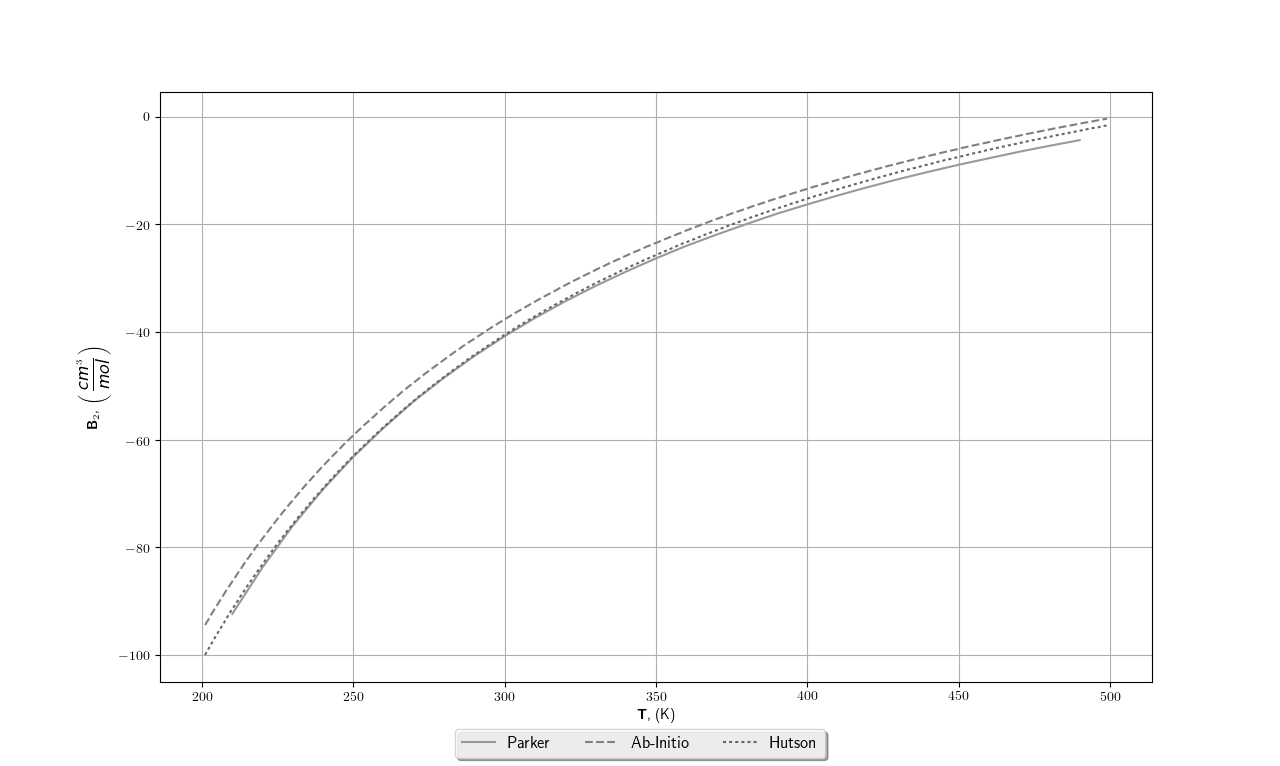
\includegraphics[width=\linewidth]{pictures/vir2.png}
\caption{Температурные зависимости вириальных коэффициентов для разных поверхностей потенциальной энергии. }
\end{figure}

\subsection{Квантовые поправки ко второму вириальному коэффициенту}

Оценка вириальных коэффициентов чисто квантовомеханическими методами существенно сложнее классических методов, поэтому был развит метод расчета квантовомеханических эффектов на основе классического приближения \cite{meyson}. Существует довольно большое количество математических методов, реализующих полуклассический подход, идея которого состоит в получении разложения вириального коэффициента по степеням постоянной Планка $\hbar$. Метод, предложеный Вигнером, позднее модифицированный Кирквудом, известен как разложение Вигнера-Кирквуда. Особенностью этого разложения является то, что в нем имеются только четные степени $\hbar$, и, таким образом, врыражения для вириальных коэффициентов представляют собой ряды по $\hbar^2$. Разложение Вигнера-Кирквуда, включая квантовые поправки на поступательное и вращательное движение (обозначаемые соответственно индексами $t$ и $r$), имеет вид
\vverh
\begin{gather}
	B = B_{\text{класс.}} + \frac{\hbar^2}{m} B_{t1} + \lb \frac{\hbar^2}{m} \rb^2 B_{t2} + \dots + \frac{\hbar^2}{I} B_{r1} + \lb \frac{\hbar^2}{I} \rb^2 B_{r2} + \dots \notag
\end{gather}

Строго разложение применимо только к существенно линейным молекулам, т.к. содержит только один момент инерции. Поправки в разложении Вигнера-Кирквуда имеют вид (для потенциала $U = U(r, \theta_1, \theta_2, \phi_2 - \phi_1)$) 
\vverh
\begin{gather}
	B_{t1} = \frac{N_0}{48 \lb kT \rb^3} \int_{0}^{\infty} \int_{\lb \Omega \rb} \exp \lb -\frac{U}{k T} \rb \lb \frac{\partial U}{\partial r} \rb^2 r^2 d r d \Omega, \notag \\
	B_{r1} = \frac{N_0}{96 \lb kT \rb^3} \int_{0}^{\infty} \int_{\lb \Omega \rb} \exp \lb -\frac{U}{k T} \rb \left[ \lb \frac{\partial U}{\partial \theta_1} \rb^2 + \lb \frac{\partial U}{\partial \theta_2} \rb^2 + \frac{1}{\sin^2 \theta_1} \lb \frac{\partial U}{\partial \phi_1} \rb^2 + \frac{1}{\sin^2 \theta_2} \lb \frac{\partial U}{\partial \phi_2} \rb^2 \right] r^2 d r d \Omega, \notag 
\end{gather}
где
\begin{gather}
	\int_{\lb \Omega \rb} d \Omega = \int_0^\pi \sin \theta_1 d \theta_1 \int_0^\pi \sin \theta_2 d \theta_2 \int_0^{2 \pi} d \lb \phi_2 - \phi_1 \rb. \notag
\end{gather}

Применительно к системе $Ar-CO_2$ получаем следующие выражения для квантовых поправок:
\vverh
\begin{gather}
	B_{1t} = \frac{\pi N_0}{12 \lb k T \rb^3} \int_0^\infty \int_0^\pi \exp \lb - \frac{U}{k T} \rb \lb \frac{\partial U}{\partial r} \rb^2 r^2 \sin \theta d r d \theta, \notag \\
	B_{1r} = \frac{\pi N_0}{24 \lb k T \rb^3} \int_0^\infty \int_0^\pi \exp \lb - \frac{U}{k T} \rb \lb \frac{\partial U}{\partial \theta} \rb^2 r^2 \sin \theta d r d \theta. \notag
\end{gather}

Поправки более высокого уровня учитывать не будем, таким образом получаем следующее выражение для вириального коэффициентов с учетом поправок первого порядка
\vverh
\begin{gather}
	B = B_{\text{класс.}} + B_{r1} + B_{t1} \notag
\end{gather}

